\documentclass{beamer}
\usepackage{listings}
\usepackage{parskip}
\lstset{
%language=C,
frame=single, 
breaklines=true,
columns=fullflexible
}

\usepackage{subcaption}
\usepackage{url}
\usepackage{tikz}
\usepackage{tkz-euclide} % loads  TikZ and tkz-base
%\usetkzobj{all}
\usetikzlibrary{calc,math}
\usepackage{float}
\newcommand\norm[1]{\left\lVert#1\right\rVert}
\providecommand{\pr}[1]{\ensuremath{\Pr\left(#1\right)}}
\renewcommand{\vec}[1]{\mathbf{#1}}
\usepackage[export]{adjustbox}
\usepackage[utf8]{inputenc}
\usepackage{amsmath}
\usetheme{Boadilla}

% # kapila students go most to acads - conclusion
% amongst ug, pg, pgs, amount of study is similar (#hrs)
%
%
% hypothesis - ug, pg no. of study hrs 
% alone and grp study comparisoin
% comparison of study hrs of ppl eating snacks vs not eating snacks

\title[MA4240 - Applied Statistics]{Intricacies of Study Environments at IIT Hyderabad}
\subtitle{MA4240 - Applied Statistics}

\author[Group Project No: 3]{Prakhar~Patni \and 
  K N~Vardhan \and
  Varunaditya~Singhal \and \\
  Tanmay~Goyal \and
  Tanay~Yadav \and
  Sujal}
\date{\today}
\begin{document}

\begin{frame}
\titlepage
\end{frame}

% \title[MA4240 - Applied Statistics]{Intricacies of Study Environments at IIT Hyderabad}
% \author[Group Project No: 3]{}
% \begin{frame}
% \titlepage
% \end{frame}

% Presentation Structure
\begin{frame}{Outline}
    \begin{enumerate}
    \item{Introduction}
    \item{Data Visualization}
    \item{Data Analysis and Conclusions}
\end{enumerate}
\end{frame}


\begin{frame}
\frametitle{Introduction}
\begin{block}{}
This project is based on the behavioral patterns of students studying at IITH. The vision was to see the changes that happened in the academic structure of our college after the strike of the pandemic, as well as how the students are dealing and coping with it. No. of study hours, preference of place, and material of studies were a few of the most common queries we asked. We use Statistics to deduce conclusions from the given data, assuming that the data is a random population sample.
\end{block}
\end{frame}

\begin{frame}
\begin{block}{Variables of interest}
\begin{enumerate}
\item Where do you like to study?
\item Gender?
\item Do you prefer to study alone?
\item How many hours do you study in one go?
\item Do you prefer snacks while studying?
\item In which block you stay?
\item Do you prefer to study on bed or study table?
\item Which program are you enrolled in?
\item Which department are you in?
\item Do you prefer live lectures or recording?
\item Do you prefer to study with lecture recording or lecture slides?
\end{enumerate}
\end{block}
\end{frame}

\begin{frame}
\begin{block}{Data Analysis Tools}
We used NumPy, Pandas, and Matplotlib modules in Python for data analysis, data cleaning (and pre-processing), and data plotting respectively.
\end{block}
\end{frame}

\begin{frame}
\begin{block}{Pre-Processing of Data}
The following steps were taken to pre-process the data:
\begin{enumerate}
    \item We began by removing white-spaces and dropping columns not required for further analysis.
    \item Since the names of the Hostel Blocks were to be an important variable for our comparisons, all entries not having the Hostel Block name were dropped.
    \item Any existing \texttt{NaNs} were replaced with the modal values of the specific column, since we do not have any model to predict the unentered values.
    \item The \textit{Hostel Block} names were replaced with their letters and the \textit{Department} names with their departmental codes.
    \item Finally, to make the data more interpretable, we assumed that any person studying between $n$ and $n+1$ hours would be studying $n + \frac{1}{2}$ hours on average.
\end{enumerate}
\end{block}
    
\end{frame}

\begin{frame}
\frametitle{Data Visualization}
\begin{block}{Analyzing the Uni-variate Numerical dataset}
\begin{center}
\captionof{table}{How many hours do you study in one go? (in hours)}
\begin{tabular}{|c|c|}
\hline 
Count & 118(non-null) \\ 
\hline 
Mean & 2.466102 \\ 
\hline 
Median & 2.5 \\ 
\hline 
Mode & 2.5 \\ 
\hline 
std & 1.246754 \\ 
\hline 
min & 1.5 \\ 
\hline 
25\% & 1.5 \\ 
\hline 
50\% & 2.5 \\ 
\hline 
75\% & 2.5 \\ 
\hline 
max & 7.5 \\ 
\hline
95\% Confidence Interval & (2.238819810180139, 2.69338357965037) \\ 
\hline
99\% Confidence Interval & (2.1656101375328065, 2.766593252297702) \\ 
\hline
\end{tabular} 
\end{center}
\end{block}
\end{frame}

\begin{frame}
\begin{block}{Visualizing the Uni-variate Numerical dataset}
\begin{figure}[hbtp]
\caption{plot of uni-variate numerical dataset}
\centering
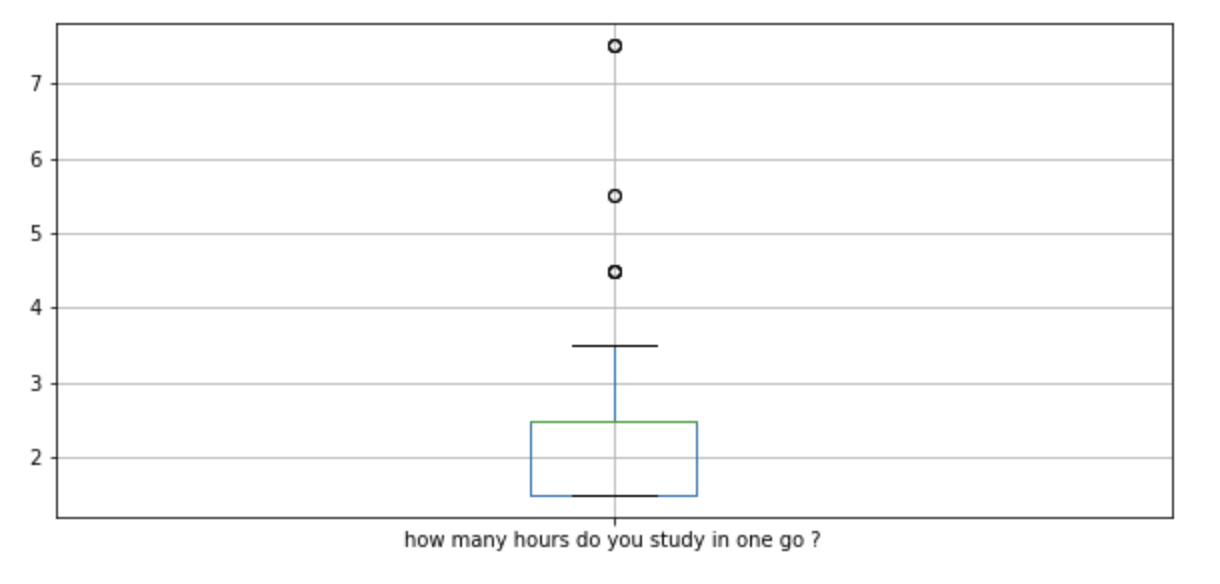
\includegraphics[scale=0.55]{output3.1.png}
\end{figure}
\end{block}
\end{frame}

\begin{frame}
\begin{block}{Visualizing the Uni-variate Numerical dataset}
\begin{figure}[hbtp]
\caption{plot of uni-variate numerical dataset}
\centering
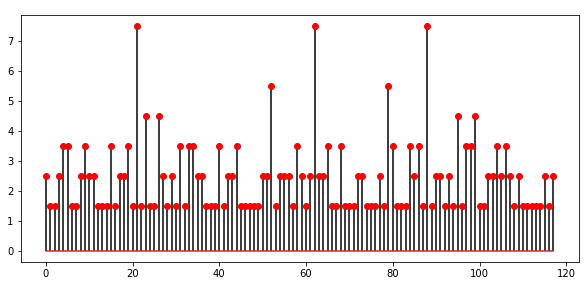
\includegraphics[scale=0.55]{output3.2.png}
\end{figure}
\end{block}
\end{frame}

\begin{frame}
\begin{block}{Data Visualization of Numerous Categorical Datasets}
\begin{figure}[hbtp]
\caption{Counts to visualize the data of study place preference}
\centering
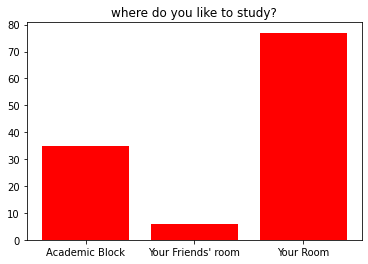
\includegraphics[scale=0.60]{wherestudy.png}
\end{figure}
\end{block}
\end{frame}

\begin{frame}
\begin{block}{Data Visualization of Numerous Categorical Datasets}
\begin{figure}[hbtp]
\caption{Counts to visualize the data of studying with friend/group or alone}
\centering
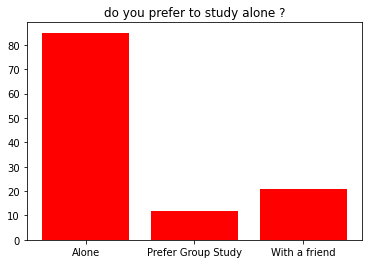
\includegraphics[scale=0.60]{study alone.png}
\end{figure}
\end{block}
\end{frame}

\begin{frame}
\begin{block}{Data Visualization of Numerous Categorical Datasets}
\begin{figure}[hbtp]
\caption{Counts to visualize the data of number of hours they study at one go}
\centering
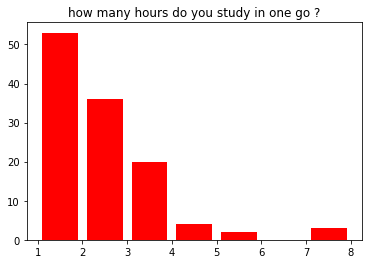
\includegraphics[scale=0.60]{hours in one go.png}
\end{figure}
\end{block}
\end{frame}

\begin{frame}
\begin{block}{Data Visualization of Numerous Categorical Datasets}
\begin{figure}[hbtp]
\caption{Counts to visualize the data of snacks preference while studying}
\centering
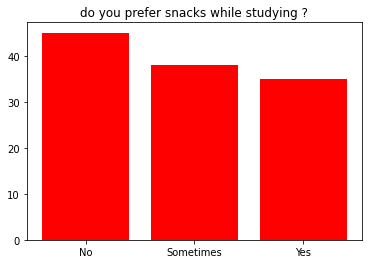
\includegraphics[scale=0.60]{snacks.png}
\end{figure}
\end{block}
\end{frame}

\begin{frame}
\begin{block}{Data Visualization of Numerous Categorical Datasets}
\begin{figure}[hbtp]
\caption{Counts to visualize the data of hostel block residence}
\centering
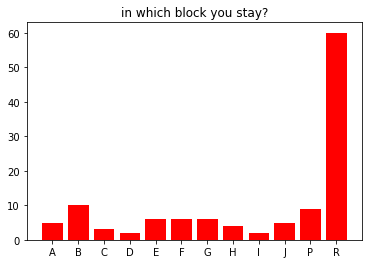
\includegraphics[scale=0.60]{block.png}
\end{figure}
\end{block}
\end{frame}

\begin{frame}
\begin{block}{Data Visualization of Numerous Categorical Datasets}
\begin{figure}[hbtp]
\caption{Counts to visualize the data of preference of study on study table or bed}
\centering
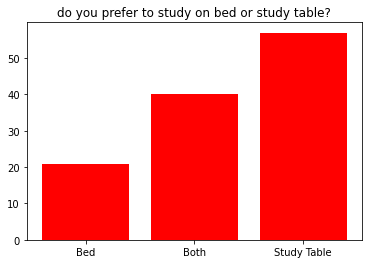
\includegraphics[scale=0.60]{bedtable.png}
\end{figure}
\end{block}
\end{frame}

\begin{frame}
\begin{block}{Data Visualization of Numerous Categorical Datasets}
\begin{figure}[hbtp]
\caption{Counts to visualize the data of program enrolled in IITH}
\centering
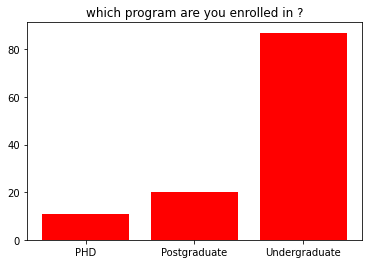
\includegraphics[scale=0.60]{program.png}
\end{figure}
\end{block}
\end{frame}

\begin{frame}
\begin{block}{Data Visualization of Numerous Categorical Datasets}
\begin{figure}[hbtp]
\caption{Counts to visualize the data of department of study}
\centering
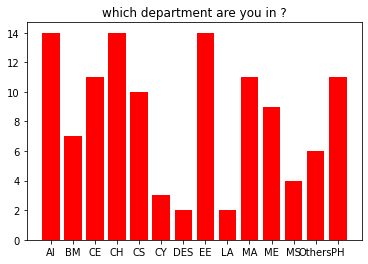
\includegraphics[scale=0.60]{department.png}
\end{figure}
\end{block}
\end{frame}

\begin{frame}
\begin{block}{Data Visualization of Numerous Categorical Datasets}
\begin{figure}[hbtp]
\caption{Counts to visualize the data live lectures preference}
\centering
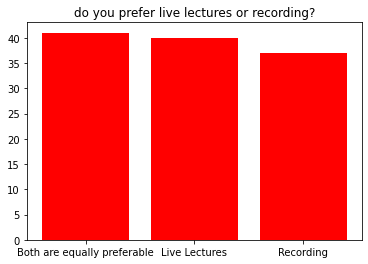
\includegraphics[scale=0.60]{reclivelec.png}
\end{figure}
\end{block}
\end{frame}

\begin{frame}
\begin{block}{Data Visualization of Numerous Categorical Datasets}
\begin{figure}[hbtp]
\caption{Counts to visualize the data of recordings/slides preference}
\centering
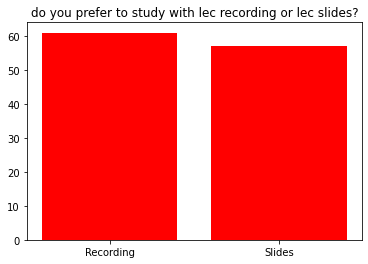
\includegraphics[scale=0.60]{recslides.png}
\end{figure}
\end{block}
\end{frame}

\begin{frame}
\begin{block}{Data Visualization with Segmented Bar plots}
\begin{figure}[hbtp]
\caption{Categorical variables in a segmented bar plot}
\centering
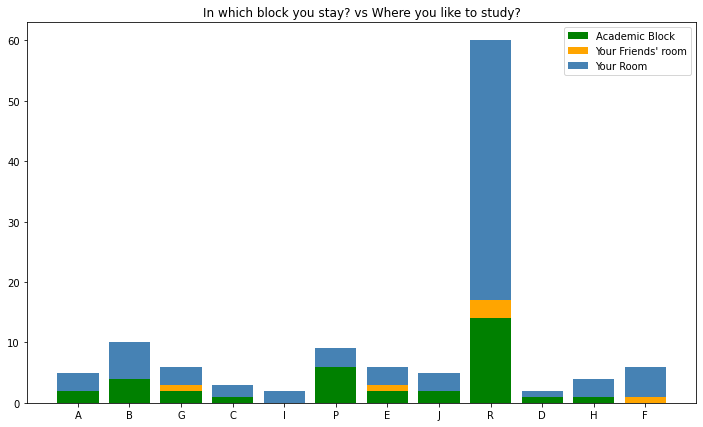
\includegraphics[scale=0.45]{output2.png}
\end{figure}
\end{block}
\end{frame}

\begin{frame}
\begin{block}{Data Visualization with Segmented Bar plots}
\begin{figure}[hbtp]
\caption{Categorical variables in a segmented bar plot}
\centering
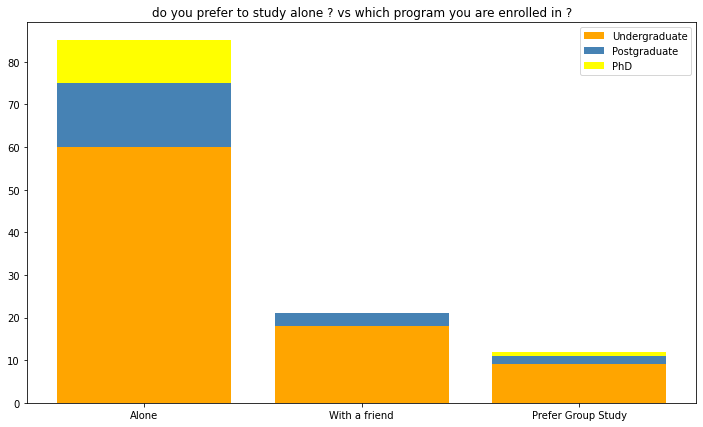
\includegraphics[scale=0.45]{output4.png}
\end{figure}
\end{block}
\end{frame}

\begin{frame}
\begin{block}{Data Visualization with Segmented Bar plots}
\begin{figure}[hbtp]
\caption{Categorical variables in a segmented bar plot}
\centering
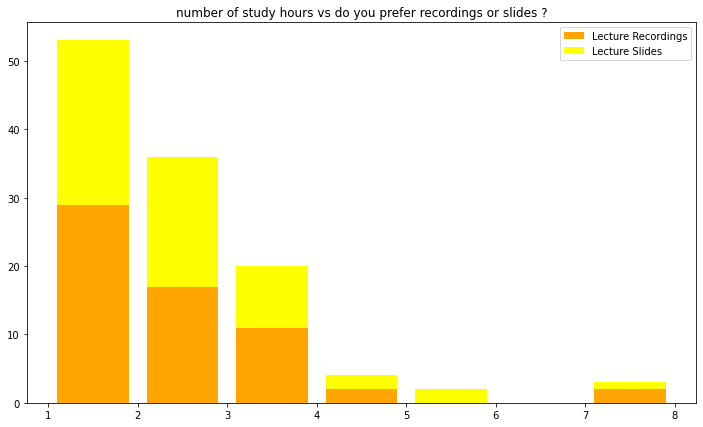
\includegraphics[scale=0.45]{output5.png}
\end{figure}
\end{block}
\end{frame}

\begin{frame}
\begin{block}{Data Visualization with Segmented Bar plots}
\begin{figure}[hbtp]
\caption{Categorical variables in a segmented bar plot}
\centering
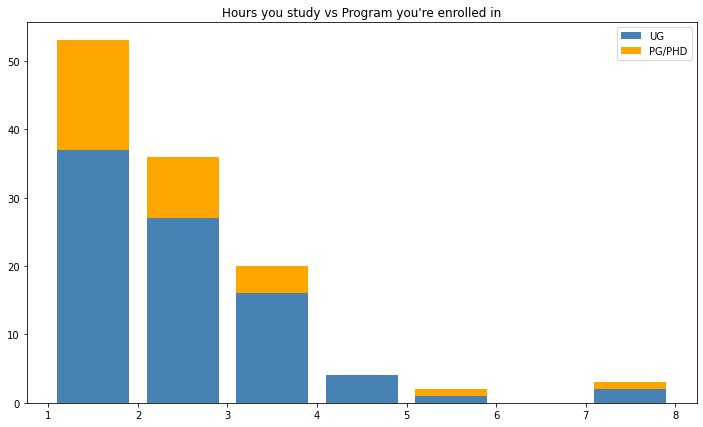
\includegraphics[scale=0.45]{hoursprogram.png}
\end{figure}
\end{block}
\end{frame}

\begin{frame}
\begin{block}{Data Visualization with Segmented Bar plots}
\begin{figure}[hbtp]
\caption{Categorical variables in a segmented bar plot}
\centering
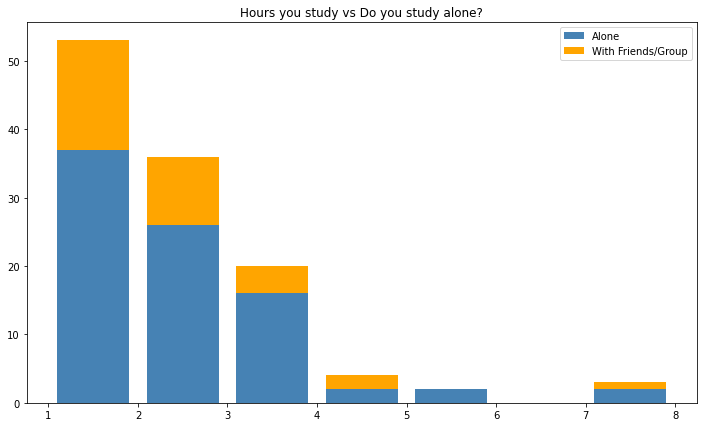
\includegraphics[scale=0.45]{hoursalone.png}
\end{figure}
\end{block}
\end{frame}

\begin{frame}
\begin{block}{Data Visualization with Segmented Bar plots}
\begin{figure}[hbtp]
\caption{Categorical variables in a segmented bar plot}
\centering
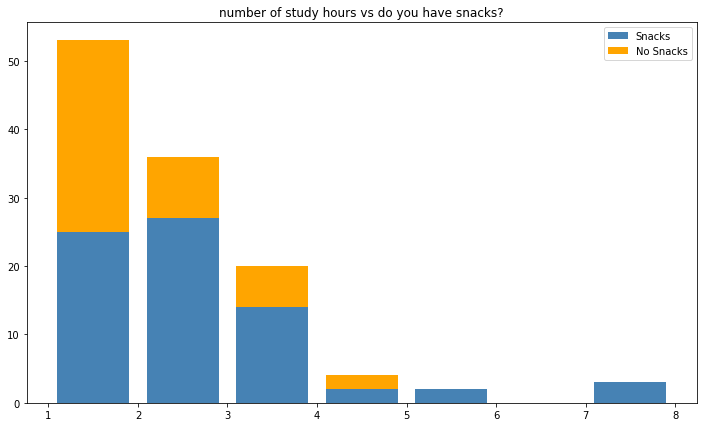
\includegraphics[scale=0.45]{snackstudytime.png}
\end{figure}
\end{block}
\end{frame}

\begin{frame}
\begin{block}{Data Visualization with Contingency Table}
\begin{figure}[hbtp]
\caption{Percentage Contingency table}
\centering
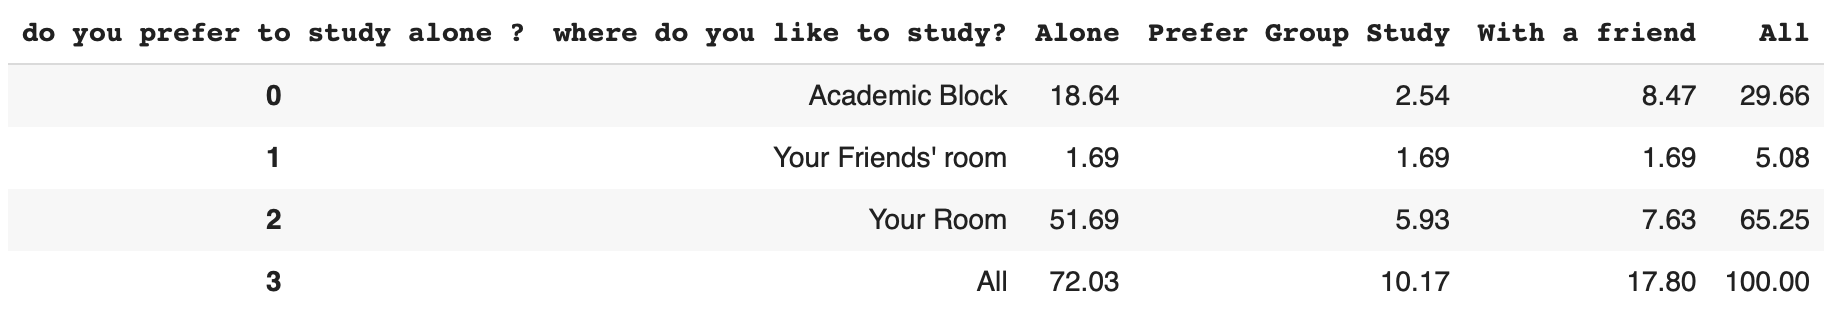
\includegraphics[scale=0.35]{output6.png}
\end{figure}
\end{block}
\end{frame}

\begin{frame}
\begin{block}{Inference}
\begin{enumerate}
\item 51.69\% people prefer to study alone in room.
\item While 18.64\% people prefer to study alone in Academic Blocks.
\item And a very few percentage of people, i.e., 1.69\% prefer to study in their friend's room.
\end{enumerate}
\end{block}
\end{frame}

\begin{frame}
\frametitle{Data Analysis and Conclusions}
\begin{block}{Uni-variate Numerical Dataset}
With around 118 students participating in the survey, we get to see that the average time (in hours) the students study at one go is around 2.46 hours, i.e., $\mu = 2.466$ hrs with a standard deviation of 1.24, i.e., $\sigma = 1.246$ hrs, and median, mode being 2.5 hours.\par
And the confidence intervals for 95\% and 99\% are,
\begin{center}
    95\% C.I - (2.239, 2.693) \\
    99\% C.I - (2.166, 2.767)
\end{center}
\end{block}
\end{frame}

\begin{frame}{Hypothesis Testings}
\begin{block}{Case 1: Comparing the study hours for Undergraduates and Postgraduates}
For Hypothesis Testing, we make the following statements - 
$ H_0 : \mu_1 - \mu_2 \geq 0$ and $H_a : \mu_1 - \mu_2 < 0$. Now, 
\par
\begin{center}
    $\bar{x_1} = 2.5$ hours \quad $\bar{x_2} = 2.43$ hours \\
    $S^2_1 = 0.5$ \quad
    $S^2_2 = 0.629$ \\
    $n_1 = 81$ \quad
    $n_2 = 37$
\end{center}

Since $\cfrac{S_1^2}{S_2^2} = 1.258 < 4$, we can assume the population variances would be equal.
\end{block}
\end{frame}

\begin{frame}{Hypothesis Testings}
\begin{block}{Case 1: Continued}
The degrees of freedom, $df = n_1 + n_2 -2 = 116$, and the pooled variance will be:
 \begin{align}
     S_p^2 &= \cfrac{(n_1-1)S_1^2 + (n_2-1)S_2^2}{n_1+n_2-2} = 1.255
 \end{align}
The test statistic $t$ is then given by:
\begin{align}
      t = 0.584
 \end{align}
Using the rejection region approach, we reject $H_0$ if $t \leq -t_{0.05, 116}$, where $t_{0.05,116} = -1.658$.\\ 
 Because the observed value of $t=0.584$ is less than $1.658$, we have enough statistical evidence to reject the null hypothesis, and thus, we can say, the postgraduates study more in one go than the undergraduates on average.
\end{block}
\end{frame}

\begin{frame}{Hypothesis Testings}
\begin{block}{Case 2: Comparing the study hours of people who study alone and who study in groups}
For Hypothesis Testing, we make the following statements - $ H_0 : \mu_1 - \mu_2 \geq 0$ and $H_a : \mu_1 - \mu_2 < 0$
\par
\begin{center}
    $\bar{x_1} = 2.488$ hours \quad $\bar{x_2} = 2.409$ hours \\
    $S^2_1 = 0.535$ \quad
    $S^2_2 = 0.647$ \\
    $n_1 = 85$ \quad
    $n_2 = 33$
\end{center}
Since $\cfrac{S_1^2}{S_2^2} = 1.209 < 4$, we can assume the population variances would be equal.
\end{block}
\end{frame}

\begin{frame}{Hypothesis Testings}
\begin{block}{Case 2: Continued}
The degrees of freedom, $df = n_1 + n_2 -2 = 116$, and the pooled variance will be:
 \begin{align}
     S_p^2 &= \cfrac{(n_1-1)S_1^2 + (n_2-1)S_2^2}{n_1+n_2-2} = 0.5658
 \end{align}
The test statistic $t$ is then given by:
\begin{align}
      t = 0.512
 \end{align}
Using the rejection region approach, we reject $H_0$ if $t \leq -t_{0.05, 116}$, where $t_{0.05,116} = -1.658$.\\ 
 Because the observed value of $t=0.512$ is less than $1.658$, we have enough statistical evidence to reject the null hypothesis, and thus, we can say, those who study in groups study more on average in one go than those who study alone.
\end{block}
\end{frame}

\begin{frame}{Hypothesis Testings}
\begin{block}{Case 3: Comparing the study hours of people who study while eating snacks and who study
without eating snacks}
For Hypothesis Testing, we make the following statements - $ H_0 : \mu_1 - \mu_2 \geq 0$ and $H_a : \mu_1 - \mu_2 < 0$
\par
\begin{center}
    $\bar{x_1} = 2.671$ hours \quad $\bar{x_2} = 2.379$ hours \\
    $S^2_1 = 0.91$ \quad
    $S^2_2 = 0.4$ \\
    $n_1 = 35$ \quad
    $n_2 = 83$
\end{center}
Since $\cfrac{S_1^2}{S_2^2} = 2.275 < 4$, we can assume the population variances would be equal.
\end{block}
\end{frame}

\begin{frame}{Hypothesis Testings}
\begin{block}{Case 3: Continued}
The degrees of freedom, $df = n_1 + n_2 -2 = 116$, and the pooled variance will be:
 \begin{align}
     S_p^2 &= \cfrac{(n_1-1)S_1^2 + (n_2-1)S_2^2}{n_1+n_2-2} = 0.55
 \end{align}
The test statistic $t$ is then given by:
\begin{align}
      t = 1.9685
 \end{align}
Using the rejection region approach, we reject $H_0$ if $t \leq -t_{0.05, 116}$, where $t_{0.05,116} = -1.658$.\\ 
Because the observed value of $t=1.9685$ is greater than $1.658$, we fail to reject the null hypothesis, and thus, do not have enough evidence to say that those who do not eat snacks while studying study for longer at one go than those who do not.
\end{block}
\end{frame}

\begin{frame}{Hypothesis Testings}
\begin{block}{Case 4: Comparing the study hours of people who study from Lecture Slides and those
who study from Lecture Recordings}
For Hypothesis Testing, we make the following statements - $ H_0 : \mu_1 - \mu_2 \geq 0$ and $H_a : \mu_1 - \mu_2 < 0$
\par
\begin{center}
    $\bar{x_1} = 2.5$ hours \quad $\bar{x_2} = 2.43$ hours \\
    $S^2_1 = 0.5$ \quad
    $S^2_2 = 0.629$ \\
    $n_1 = 57$ \quad
    $n_2 = 61$
\end{center}
Since $\cfrac{S_1^2}{S_2^2} = 1.258 < 4$, we can assume the population variances would be equal.
\end{block}
\end{frame}

\begin{frame}{Hypothesis Testings}
\begin{block}{Case 4: Continued}
The degrees of freedom, $df = n_1 + n_2 -2 = 116$, and the pooled variance will be:
 \begin{align}
     S_p^2 &= \cfrac{(n_1-1)S_1^2 + (n_2-1)S_2^2}{n_1+n_2-2} = 0.5764
 \end{align}
The test statistic $t$ is then given by:
\begin{align}
      t = 0.5
 \end{align}
Using the rejection region approach, we reject $H_0$ if $t \leq -t_{0.05, 116}$, where $t_{0.05,116} = -1.658$.\\ 
Because the observed value of $t=0.5$ is lesser than $1.658$,we have enough statistical evidence to reject the null hypothesis, and thus, we can say, those who study from recordings study more on average in one go than those who study from slides.
\end{block}
\end{frame}

\title{THANK YOU}
\author[]{}
\begin{frame}
    \maketitle
\end{frame}

\end{document}
